\section{Identyfikacja parametrów systemu}
Punktem wyjściowym do rozpoczęcia prac był laboratoryjny model wahadła zbudowany w Simulinku mający następujące sygnały:\\
Wejściowe: sygnał sterujący podawany na silnik (zakres: -0.5 do 0.5), reset enkoderów.\\
Wyjściowe: odczytane z enkoderów położenie kątowe wahadła oraz położenia wózka na szynie, prędkość kątowa wahadła oraz prędkość wózka na szynie (obliczone jako iloraz różnicowy położenia w czasie).\\ 
Przyjęto, że punkt nieciągłości położenia wahadła będzie znajdował się w dolnym, stabilnym położeniu równowagi, natomiast enkodery resetowane będą w lewym (patrząc od strony komputera) skrajnym położeniu wózka na szynie.
\subsection{Obliczenie momentu bezwładności wahadła}
Wahadło składa się z rurki oraz ciężarka znajdującego się na jej końcu. Rozkręcając wahadło zważono oraz zmierzono niezbędne wielkości potrzebne do analitycznego wyliczenia momentu bezwładności wahadła.\\
\noindent\rule[0.2cm]{\textwidth}{1pt}
Masa rurki $m_r=0.02[kg]$\\
Masa ciężarka $m_c=0.011[kg]$\\
Całkowita długość wahadła $d_w=0.495[m]$\\
Odległość od początku rurki do osi obrotu $d_1=0.085[m]$\\
Odległość od osi obrotu do środka masy wahadła $l=0.252[m]$.\\
\noindent\rule[0.5cm]{\textwidth}{1pt}
Rozważając rurkę jako nieskończenie cienki pręt oraz ciężarek jak masę punktową obliczono moment bezwładności wahadła względem osi obrotu: 
\begin{equation}
J_{os} = 2(\frac{m_r}{3}(\frac{d_w-d_1}{d_w}(d_w-d_1)^2+\frac{d_1}{d_w}d_1^2)+m_c(d_w-d_1)^2)
\end{equation}
Na stanowisku wahadło składa się z dwóch identycznych części, stąd współczynnik 2. Po podstawieniu wartości $J_{os} = 0.00557 [kg \cdot m^2]$.\\
Uzyskany wynik postanowiono porównać z wynikiem eksperymentalnym. Unieruchomiwszy wózek nieznacznie wychylono wahadło i zarejestrowano drgania w czasie.  Zmierzono średni okres drgań $T = 1.207s$. Traktując obiekt jako wahadło fizyczne wyliczono moment bezwładności $J_{eksp}$ według znanej zależności:
\begin{equation}
T = 2\pi\sqrt{\dfrac{J_{eksp}}{2(m_c+m_r)gl}}
\end{equation}
gdzie g oznacza przyspieszenie ziemskie.
Otrzymano wynik $J_{eksp} = 0.00565 [kg \cdot m^2]$ zadowalająco bliski analitycznemu.

Aby uprościć model matematyczny systemu policzono moment bezwładności $J_{sm}$ wahadła względem jego środka masy. Wykorzystano twierdzenie Steinera:
\begin{equation}
J_{os} = J_{sm} + 2\cdot(m_c+m_r)\cdot l^2
\end{equation}
Skąd ostatecznie $J_{sm} = 0.00167[kg \cdot m^2]$.
\subsection{Identyfikacja modelu dynamiki wózka}
Przyjmując uproszczony model silnika DC zapisano następujący układ równań:
\begin{align}
u &= Ri + k_e\omega \\
J_{DC}\dot{\omega} &= k_mi - \mu\omega
\end{align}
gdzie:\\
u - napięcie podane na silnik,\\
R - rezystancja wirnika,\\
i - natężenie prądu,\\
$\omega$ - prędkość kątowa wirnika,\\
$k_e$ - stała elektryczna silnika,\\
$k_m$ - stała mechaniczna silnika,\\
$J_{DC}$ - moment bezwładności układu względem osi obrotu silnika.\\
$\mu$ - wypadkowy współczynnik tarcia układu\\
Eliminując \textit{i}:
\begin{equation}
\label{eq:dynW}
\dot{\omega}=-\frac{k_ek_m+\mu R}{J_{DC}R}\omega+\frac{k_m}{J_{DC}R}u
\end{equation}
Aby uniknąć konieczności wyznaczania wszystkich wielkości występujących w równaniu \ref{eq:dynW} postanowiono zidentyfikować dwie stałe $c_1$ oraz $c_2$. Mając na uwadze, że prędkość wózka na szynie $\dot{z}$ jest proporcjonalna do prędkości obrotowej wirnika:
\begin{equation}
\label{eq:zz}
\ddot{z}=-c_1\dot{z}+c_2u
\end{equation}
Minimalizując całkę z kwadratu różnicy pomiędzy rzeczywistym przebiegiem a modelem opartym o wyżej wymienione stałe otrzymano rezultat:
\begin{figure}[H]
\centering
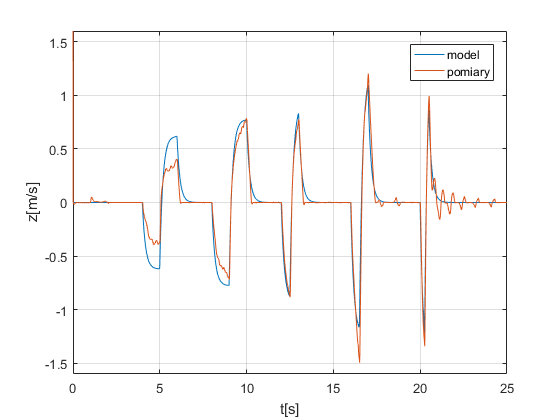
\includegraphics[width=12cm]{obrazy/pr_woz.png}
\label{fig:wozek}
\caption{Porównanie modelu dynamiki wózka z pomiarami}
\end{figure}
dla $c_1 = 5.8$, $c_2 = -18$. 

Pominięto wpływ wahadła na ruch wózka. Uproszczenie to jest szczególnie uzasadnione w momencie kiedy wahadło znajdować się będzie w niestabilnym punkcie równowagi. Na rysunku \ref{fig:wozek} widać, że przy mniejszych prędkościach występują większe rozbieżności pomiędzy modelem a pomiarami, co spowodowane jest bardziej znaczącym wpływem tarcia statycznego, którego nie uwzględniono do tej pory w modelu.
